%%%%%%%%%%%%%%%%%%%%%%%%%%%%%%%%%%%%%%%%%
% Beamer Presentation
% LaTeX Template
% Version 1.0 (10/11/12)
%
% This template has been downloaded from:
% http://www.LaTeXTemplates.com
%
% License:
% CC BY-NC-SA 3.0 (http://creativecommons.org/licenses/by-nc-sa/3.0/)
%
%%%%%%%%%%%%%%%%%%%%%%%%%%%%%%%%%%%%%%%%%

%----------------------------------------------------------------------------------------
%	PACKAGES AND THEMES
%----------------------------------------------------------------------------------------

\documentclass[t]{beamer}

\mode<presentation> {

% The Beamer class comes with a number of default slide themes
% which change the colors and layouts of slides. Below this is a list
% of all the themes, uncomment each in turn to see what they look like.

%\usetheme{default}
%\usetheme{AnnArbor}
%\usetheme{Antibes}
%\usetheme{Bergen}
%\usetheme{Berkeley}
%\usetheme{Berlin}
%\usetheme{Boadilla}
%\usetheme{CambridgeUS}
%\usetheme{Copenhagen}
%\usetheme{Darmstadt}
%\usetheme{Dresden}
%\usetheme{Frankfurt}
%\usetheme{Goettingen}
%\usetheme{Hannover}
%\usetheme{Ilmenau}
%\usetheme{JuanLesPins}
%\usetheme{Luebeck}
\usetheme{Madrid}
%\usetheme{Malmoe}
%\usetheme{Marburg}
%\usetheme{Montpellier}
%\usetheme{PaloAlto}
%\usetheme{Pittsburgh}
%\usetheme{Rochester}
%\usetheme{Singapore}
%\usetheme{Szeged}
%\usetheme{Warsaw}

% As well as themes, the Beamer class has a number of color themes
% for any slide theme. Uncomment each of these in turn to see how it
% changes the colors of your current slide theme.

%\usecolortheme{albatross}
%\usecolortheme{beaver}
%\usecolortheme{beetle}
%\usecolortheme{crane}
%\usecolortheme{dolphin}
%\usecolortheme{dove}
%\usecolortheme{fly}
%\usecolortheme{lily}
%\usecolortheme{orchid}
%\usecolortheme{rose}
%\usecolortheme{seagull}
%\usecolortheme{seahorse}
%\usecolortheme{whale}
%\usecolortheme{wolverine}

%\setbeamertemplate{footline} % To remove the footer line in all slides uncomment this line
%\setbeamertemplate{footline}[page number] % To replace the footer line in all slides with a simple slide count uncomment this line

%\setbeamertemplate{navigation symbols}{} % To remove the navigation symbols from the bottom of all slides uncomment this line
}

\usepackage{graphicx} % Allows including images
\usepackage{booktabs} % Allows the use of \toprule, \midrule and \bottomrule in tables

%----------------------------------------------------------------------------------------
%	TITLE PAGE
%----------------------------------------------------------------------------------------

\title[SAO101]{SAO101: Intro to designing PCBs in KiCad} % The short title appears at the bottom of every slide, the full title is only on the title page

\author{Josh Johnson} % Your name
\institute[] % Your institution as it will appear on the bottom of every slide, may be shorthand to save space
{ \\ % Your institution for the title page
\medskip
\textit{} % Your email address
}
\date{8/4/2019} % Date, can be changed to a custom date

\begin{document}

\begin{frame}
\titlepage % Print the title page as the first slide
\end{frame}

%----------------------------------------------------------------------------------------
%	PRESENTATION SLIDES
%----------------------------------------------------------------------------------------

\section{Subsection Example} % A subsection can be created just before a set of slides with a common theme to further break down your presentation into chunks

\begin{frame}
\frametitle{Overview}
\begin{itemize}
\item What and why?
\item Schematic Capture
\item PCB Manufacturing and Assembly
\item Design rules
\item Layout 
\item Gerber generation / file upload
\item Profit?
\end{itemize}
\vspace{30mm}
Project Files: \url{github.com/joshajohnson/CBRhardware}\\
\end{frame}

%----------------------------------------------------------------------------------------

\begin{frame}[t]
\frametitle{What's KiCad?}

	A Cross Platform and Open Source Electronic Design Automation Suite
	
	\begin{columns}
		\column{.69\textwidth}
		\begin{itemize}
			\item KiCad - project manager
			\item Eeschema – schematic capture
			\item Pcbnew - layout program
			\item GerbView - gerber viewer
			\item Bitmap2Component - import images to PCB
		\end{itemize}
		
		
		\column{.3\textwidth}
			\begin{figure}
			
\includegraphics[width=1\linewidth]{kikeycad.png}
		\end{figure}
		
	\end{columns}


\end{frame}

%----------------------------------------------------------------------------------------

\begin{frame}
\frametitle{What's a Shitty Add On?}
Cool PCBs 
\begin{columns}[c]
	\column{.5\textwidth}
	\begin{figure}
		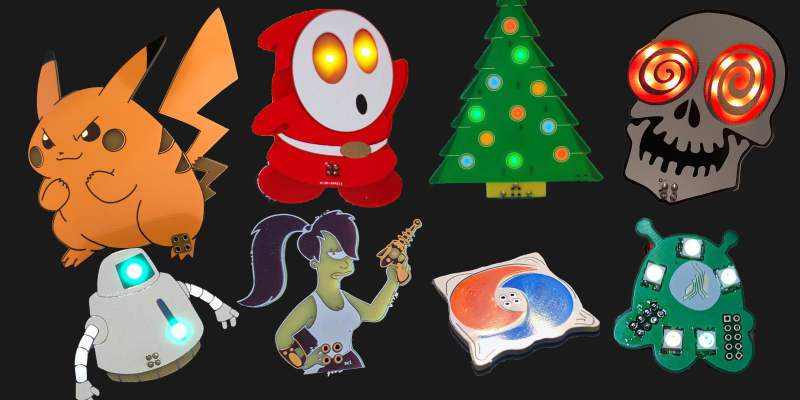
\includegraphics[width=1\linewidth]{shittyadd-ons.png}
	\end{figure}

	\begin{figure}
		
\includegraphics[width=1\linewidth]{bogan.jpg}
	\end{figure}
	
	\column{.24\textwidth}
	\begin{figure}
		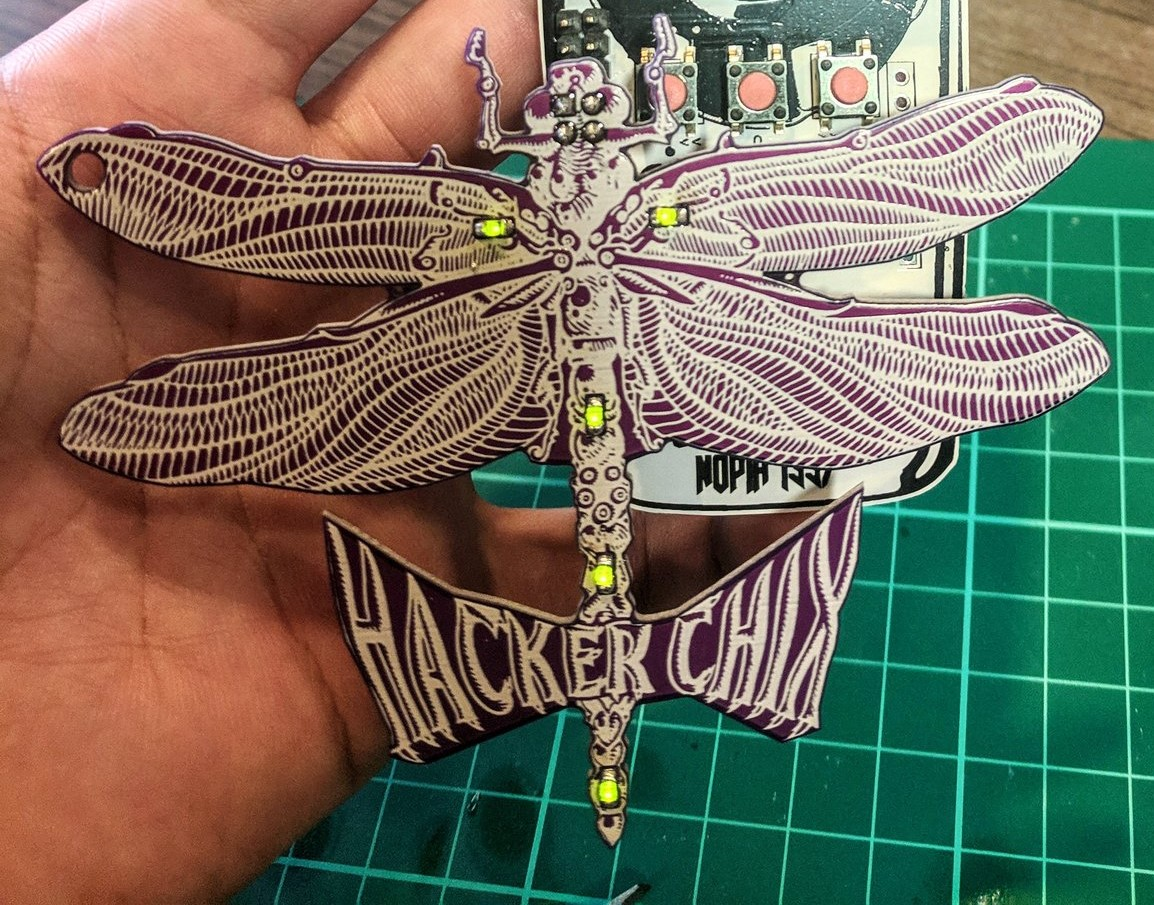
\includegraphics[width=1\linewidth]{hackerchix.jpg}
	\end{figure}
	
	\column{.24\textwidth}
	\begin{figure}
		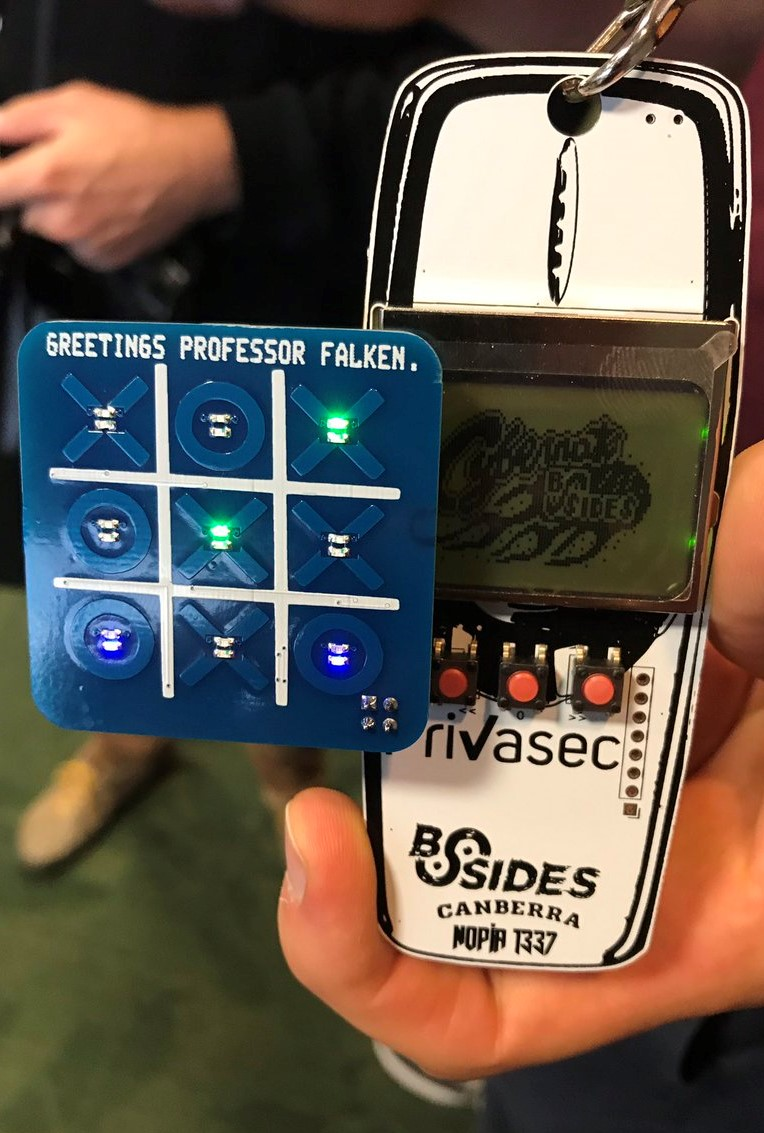
\includegraphics[width=1\linewidth]{joshsao.jpg}
	\end{figure}

\end{columns}

\end{frame}

%------------------------------------------------

\begin{frame}
\frametitle{What's a Shitty Add On?}
"Standardised" Connector
\begin{columns}[c]
	\column{.33\textwidth}
	\begin{figure}
		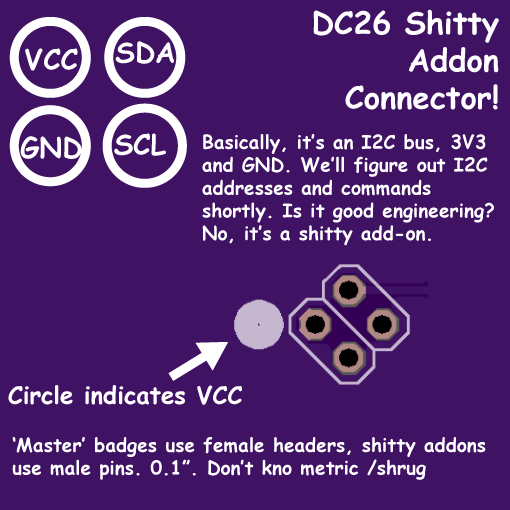
\includegraphics[width=0.9\linewidth]{sao.png}
	\end{figure}
	
	\column{.33\textwidth}
	\begin{figure}
		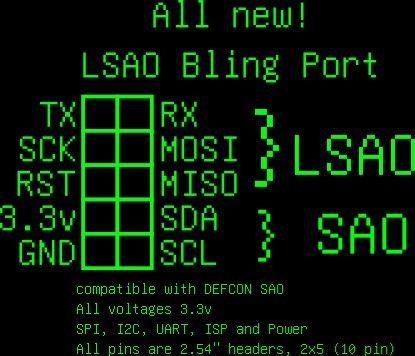
\includegraphics[width=0.9\linewidth]{LSAO.jpg}
	\end{figure}
	
	\column{.33\textwidth}
	\begin{figure}
		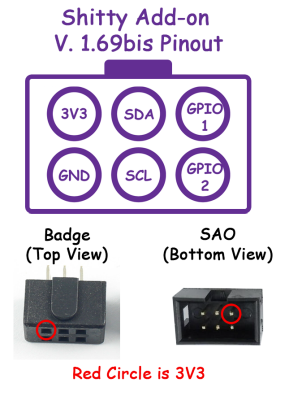
\includegraphics[width=0.9\linewidth]{sao69.png}
	\end{figure}
	
\end{columns}

https://hackaday.com/2019/03/20/introducing-the-shitty-add-on-v1-69bis-standard/
\end{frame}

%----------------------------------------------------------------------------------------

\begin{frame}
\frametitle{Today's Design}
Based around Microchip's MCP23017 I$^2$C 16 Bit I/O expander

\begin{columns}[c]
	\column{.39\textwidth}
	\begin{figure}
		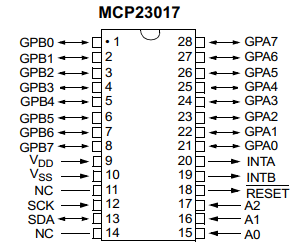
\includegraphics[width=1\linewidth]{mcp23071pinout.PNG}
	\end{figure}
	
	\column{.6\textwidth}
	\begin{figure}
		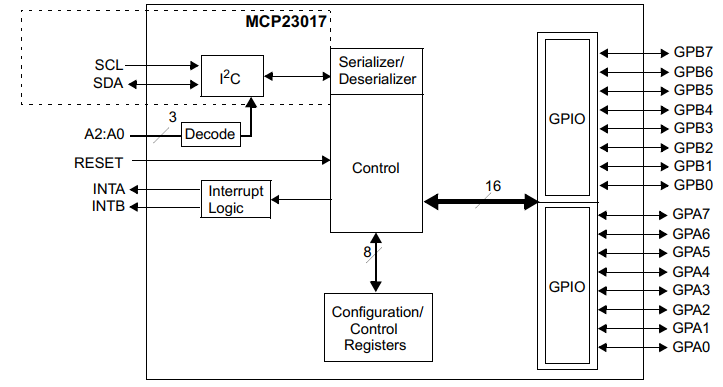
\includegraphics[width=1\linewidth]{mcpFunctional.png}
	\end{figure}
\end{columns}
\vspace{7mm}
Allows control of 16 pins with just two inputs.\\
Can connect up to 8 MCP23017's to those same two pins.\\
128 controlled pins from a single I$^2$C bus.\\

\end{frame}

%----------------------------------------------------------------------------------------

\begin{frame}
\frametitle{Schematic Capture Time!}
Enough theory, time to draw up the schematic.
\end{frame}


%----------------------------------------------------------------------------------------

\begin{frame}
\frametitle{PCB Manufacturing and Assembly Process}

\begin{figure}
	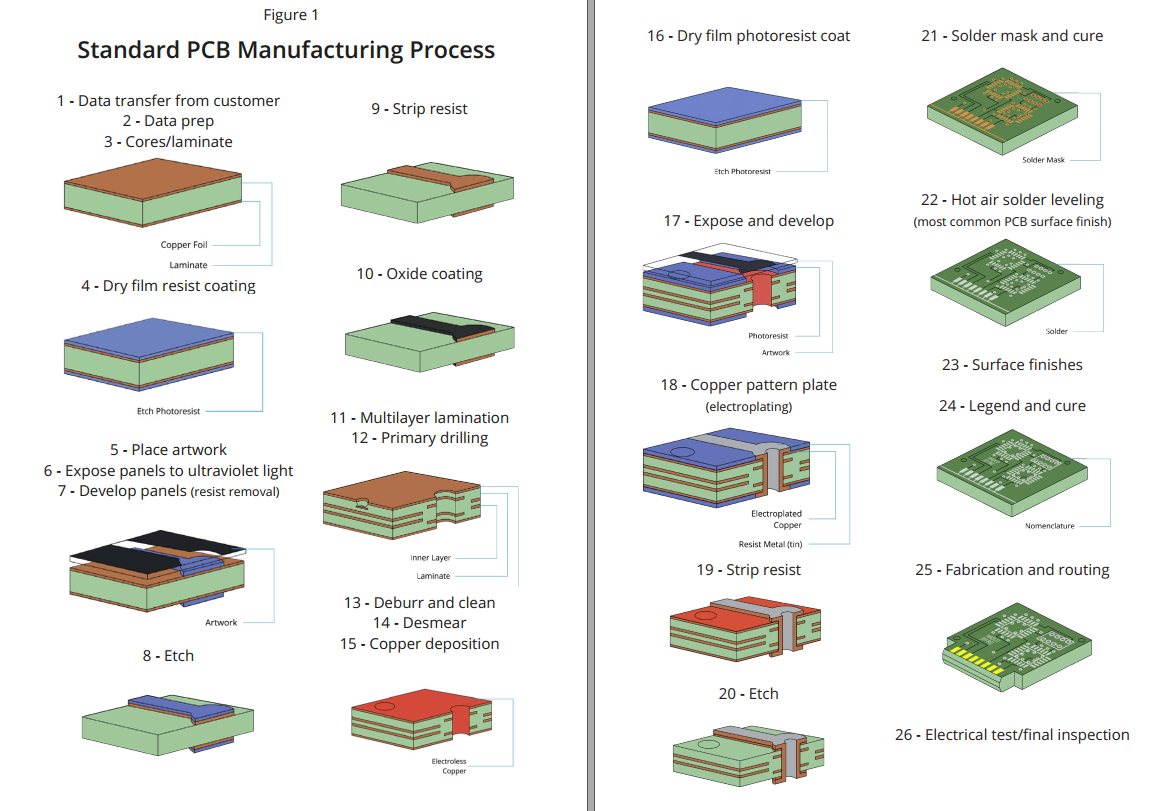
\includegraphics[width = 0.9\linewidth]{pcbManufacture.png}
\end{figure}

\end{frame}

%----------------------------------------------------------------------------------------

\begin{frame}
\frametitle{Design Rules}
Need to ensure that our board can be fabricated (at a reasonable cost).
\end{frame}

%----------------------------------------------------------------------------------------

\begin{frame}
\frametitle{Time to lay the board out!}
This is the fun part!\\

\end{frame}

%----------------------------------------------------------------------------------------

\begin{frame}
\frametitle{Want to learn more?}
Board ready to route: \texttt{uC101/RouteMe}\\
Links to resources: \texttt{SAO101/README.md}

\end{frame}

%----------------------------------------------------------------------------------------

\begin{frame}
\frametitle{Feedback}
Please let me know what you want these meetups to be. \\
\begin{itemize}
\item Workshop / Talks / Project Show \& Tell / ?
\item Suggested topics to cover
\begin{itemize}
	\item Intro to Microcontrollers / Interfacing with the real world
	\item Circuit Design
	\item Rapid Prototyping
	\item PCB Design, Manufacturing, and Assembly
	\item Intro to FPGAs
	\item Whatever you want!
\end{itemize}
\end{itemize}
\vspace{5mm}
Say Hello! \\
BSidesCbr Slack: josh\\
Twitter: @\textunderscore joshajohnson\\
Email: josh@joshajohnson.com\\
\vspace{4mm}

Project Files: \url{github.com/joshajohnson/CBRhardware}\\
\end{frame}


\end{document} 